\section{数据集和特征构造}
\label{dataset}

\subsection{数据概览}

本项工作使用的主要数据集取自《剩草量分析表》,包含第三牧场2017年3月5日至7月25日约140天的各牛棚采食情况记录。数据集包含的牛棚列举在表\ref{cowshed}中。数据集记录了16个牛棚每天的\emph{牛头数}\footnote{牛只调群很常见,因此每个牛棚每天的牛群规模可能会有增减。},\emph{报草量},\emph{减草量}\footnote{每天有一次机会可以对上报草量进行增减。例如观察到中午牛食欲不振,则可以适当减少当天至第二天的总草量。减草量也可以为负值,表示适当增加草量。},\emph{剩草量}和\emph{头均产奶量}。通过简单计算可以进一步得到计划头均采食量($r_t =$(报草量-减草量)/牛头数)和实际头均采食量($y_t =$(报草量-减草量-剩草量)/牛头数)。

\begin{table}
\caption{牛棚概览}
\label{cowshed}
\footnotesize
\begin{center}
\begin{tabular}{|c|}
\hline
	\textbf{牛棚}  \\
\hline
    B1-1N  B1-1S  
    B1-3N  B1-3S  \\
    B1-5N  B1-5S  
    B1-7N  B1-7S  \\
    B4-1N  B4-1S  
    B4-3N  B4-3S  \\
    B4-5N  B4-5S  
    B4-7N  B4-7S  \\
\hline
\end{tabular}
\end{center}
\end{table}


\emph{温度、湿度}是影响头均采食量的重要影响参数。温度和湿度数据可从记录历史天气的网站如\cite{weather,tianqi}上抓取获得\footnote{\cite{weather}上可能无湿度信息,\cite{tianqi}上有湿度信息。}。

\emph{泌乳期(胎次)}和\emph{泌乳周}(实际采用的是\emph{泌乳天数})数据可以从牧场管理系统(银香伟业采用阿菲金管理系统)中获取。这两项数据处理的细节请参考附录第\ref{calving_data}节。



\subsection{关于部分未采用数据说明} 
\begin{itemize}
\item 奶牛品种:各牧场主要包含两种奶牛:荷斯坦奶牛和娟姗奶牛(同牛棚同日内牛群属同种)。但当前第三牧场中全部牛只均为荷斯坦奶牛,无娟姗奶牛,故我们不区分牛的品种,对所有数据统一处理。

\item 奶牛体重:我们将牛棚的牛群作为整体分析其头均采食量,故暂时假设各牛棚头均体重相似,不是影响头均采食量的主要因素。

\item 奶牛运动量:当前先假设各牛棚牛群每日运动量相近。如有计步器数据,可将步数信息和采食量做关联性分析。

\item 奶牛身心状况:奶牛身心状况难以量化。目前工作未考虑此类特征。未来工作可考虑通过牧场系统中对牛的检查、治疗等事件记录推断估计出各牛棚的整体健康状态。

\item 饲料特性:各牛棚除新产牛外(?待验证),主要采用同种配方的饲料。本项工作主要针对处高产期的牛的采食量建模,故模型未将饲料相关的数据视作输入变量。

\item 其他应激:当前数据集未包含疫苗注射记录。据技术人员称疫苗注射会令牛产生应激,影响短期内采食量。未来工作可考虑通过牧场系统中对牛的检查、治疗等事件记录推断、量化每天各牛棚可能的应激事件。
\end{itemize}


\subsection{数据预处理和特征构造}

根据《剩草量分析表》中“牛只类型”字段标注,各牛棚在大部分日期内牛属于“高产”,但个别牛棚在部分日期内被标注为“新产”(生产完牛犊后处于泌乳初期的牛?)。在建模前我们将所有标注为“新产”的数据样本剔除掉。
同时部分日期的数据存在缺失值。当前我们采取最简易的缺失值处理手段:将不完整的数据样本剔除掉。


在预测第$t+1$天头均采食量$y_{t+1}$时,本工作尝试多种构建输入变量$X$的方式,主要可分为两类
(1)仅考虑第$t$天的观测情况(头均采食量、头均产奶量、温湿度),和(2)考虑到一段连续日期即$t-w, t-w+1, \cdots, t$天的观测情况,包括头均采食量、头均产奶量、连续w天头均采食量(直接拼接或用小波分解提取系数)等。对时间序列数据的处理请见第\ref{time_series}小节。

我们对于温湿度数据,计算得到THI(Thermal-Humidity Index,温湿度指数)指标作为模型的输入变量,而不是将温度和湿度作为单独的变量输入模型。THI是一个用温度和湿度的综合影响反应热应激水平的指标,它有多种不同的定义/计算方式,最常用的经验公式为:
\begin{equation}
	THI=0.72 \times (Td + Tw) + 40.6
\end{equation}
其中$Td$和$Tw$分别为干湿球温度计读出的干球温度和湿球温度。但由于干湿球温度数据不便于获取,我们在本工作中采用另一种计算THI的公式\cite{thi_cow_wang}:
\begin{equation}
	THI=0.81Td + (0.99Td - 14.3)RH + 46.3
\end{equation}
其中RH(Relative Humidity)为相对湿度。由于每天的温度是个随时间变化的变量,我们在实验中用天气预报给出的当日最高气温来代替公式中的干球温度Td,来表征牛受到热应激的情况。

在附录第\ref{calving_data}节中,我们介绍了各牛只泌乳天数、泌乳期数据的获取。由于我们以牛棚为单位进行建模,我们取各牛棚每天牛群的泌乳天数、泌乳期的\emph{中位数}\footnote{采取中位数而非平均数的动机是避免少量离群点对整体统计指标带来较大偏移。},作为对该日该牛群整体泌乳周期状态的刻划。

\subsubsection{时间序列的处理}
\label{time_series}

我们对多天历史数据采取两种处理方式:直接拼接和提取小波分解的系数作特征。我们分别考虑拼接历史头均采食量的时间序列,或者头均产奶量的时间序列\footnote{我们未同时考虑两个时间序列,因为此两时间序列有一定相关性,且实验发现拼接两个时间序列并未获得更优的测试集误差。},而对其他特征(THI、泌乳天数、胎次)不考虑历史数据。

形式化地,当我们考虑拼接头均采食量时间序列时,每条样本的形式为
\begin{equation}
	\langle (y_{t-w+1}, \cdots, y_t, m_t, T_{t+1}, cd_{t}, cp_{t}), y_{t+1} \rangle
\end{equation}
	其中$y_{t+1}$预测目标,$y_k$为某牛舍第$k$天的实际头均采食量,$m_k$为某牛棚第$k$天的头均产奶量,$T_{k}$为第$k$天的THI值(可借助天气预报获得未来一天的THI值), $cd_{k}$和$cp_{k}$分别为某牛棚第$k$天的泌乳天数和胎次的中位数。
	
类似地,当我们考虑拼接头均产奶量时间序列时,每条样本的形式为
\begin{equation}
	\langle (y_t, m_{t-w+1}, \cdots, m_t, T_{t+1}, cd_{t}, cp_{t}), y_{t+1} \rangle
\end{equation}

另一种处理历史时间序列数据的策略是离散小波分解(Discrete Wavelet Transform,DWT)。小波分解是一种常用的信号处理手段。回顾傅里叶变换将时域的信号通过变换得到了精确的频域信号,但完全丢失了时域信息。小波变换在时域精确测量和频域精确测量间做了折衷。通过小波分解,我们可得到有关信号时域和频域的一些信息。在本文中,我们采用离散小波变换(DWT)。关于小波变换的更多介绍可以参考\cite{vidakovic1994wavelets, valens1999really}和Youtube上搜索“Discrete Wavelet Transform”查询到的相关视频。

离散小波分解的过程可如示意图\ref{dwt}所示。原始信号x(长度为k序列)经过1层小波分解得到长度为k/2的1阶近似和长度为k/2的1阶细节。我们可以继续把1阶近似作为原始信号做1层离散小波分解,得到的长度为k/4的1阶近似和长度为k/4的1阶细节对于信号x而言是2阶近似和2阶细节。以此类推。

\begin{figure}
\begin{center}
	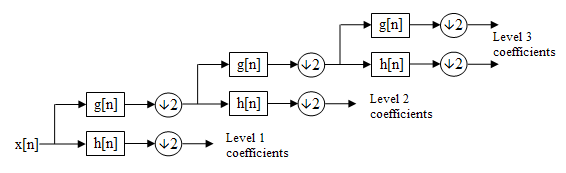
\includegraphics[width=0.95\linewidth]{dwt}
\caption{3层离散小波分解示意图。}
\label{dwt}
\end{center}
\end{figure}

在本工作中,以考虑头均采食量序列为例,我们对于长度为w的序列${y_{t-w+1}, y_{t-w+2}, \cdots, y_t}$做1阶或2阶小波分解,得到$\langle cA, cD\rangle$或$\langle cA', cD', cD\rangle$,并把它们作为特征输入给模型。其中,$cA, cD, cA', cD'$分别为小波分解的1阶近似、细节,2阶近似、细节。因而,以做1阶小波分解为例,每条样本的形式为
\begin{equation}
	\langle (y_t, cA, cD, m_t, T_{t+1}, cd_{t}, cp_{t}), y_{t+1} \rangle
\end{equation}
考虑头均产奶量序列时,对数据的处理与之类似。



数据预处理和特征提取的具体细节请参考代码文件(preprocess.ipynb和model.ipynb)中的文字说明。
不同方式构建模型的性能请见第\ref{evaluation}节。







